\section{Аналитическая часть}

\subsection{Постановка задачи}\label{sec:task}
В соответствии с заданием курсового проекта, требуется разработать загружаемый модуль ядра, позволяющий управлять устройствами, подключенными с помощью интерфейса GPIO.

Для достижения данной цели необходимо решить следующие задачи:
\begin{enumerate}
	\item проанализировать особенности интерфейса GPIO, определить формат передаваемых данных;
	\item проанализировать и выбрать тип программного управления;
	\item разработать программное обеспечение и протестировать его.
\end{enumerate}

\subsection{Анализ принципов работы интерфейса GPIO}
\textbf{GPIO} - интерфейс для связи между компонентами компьютерной системы, к примеру, микропроцессором и различными периферийными устройствами\cite{subj:def}. Контакты GPIO могут выступать как в роли входа, так и в роли выхода — это, как правило, конфигурируется. Обычно они используются для подключения датчиков, переключателей, дисплеев и т.п.

В данной работе будет использоваться одноплатный компьютер Raspberry Pi 2B ввиду отсутствия в распоряжении других компьютеров. Рассмотрим подробнее организацию GPIO на его примере.

На рисунке \ref{pic:gpio} описывается назначение каждого из контактов (пинов)  для этой модели. Можно отметить, что не все из них используются для ввода/вывода. Помимо этого есть контакты предназначенные для подачи определённого напряжения на внешние устройства (3.3V, 5V) или для заземления (GROUND).

\begin{figure}[h!] 
	\begin{center}
		{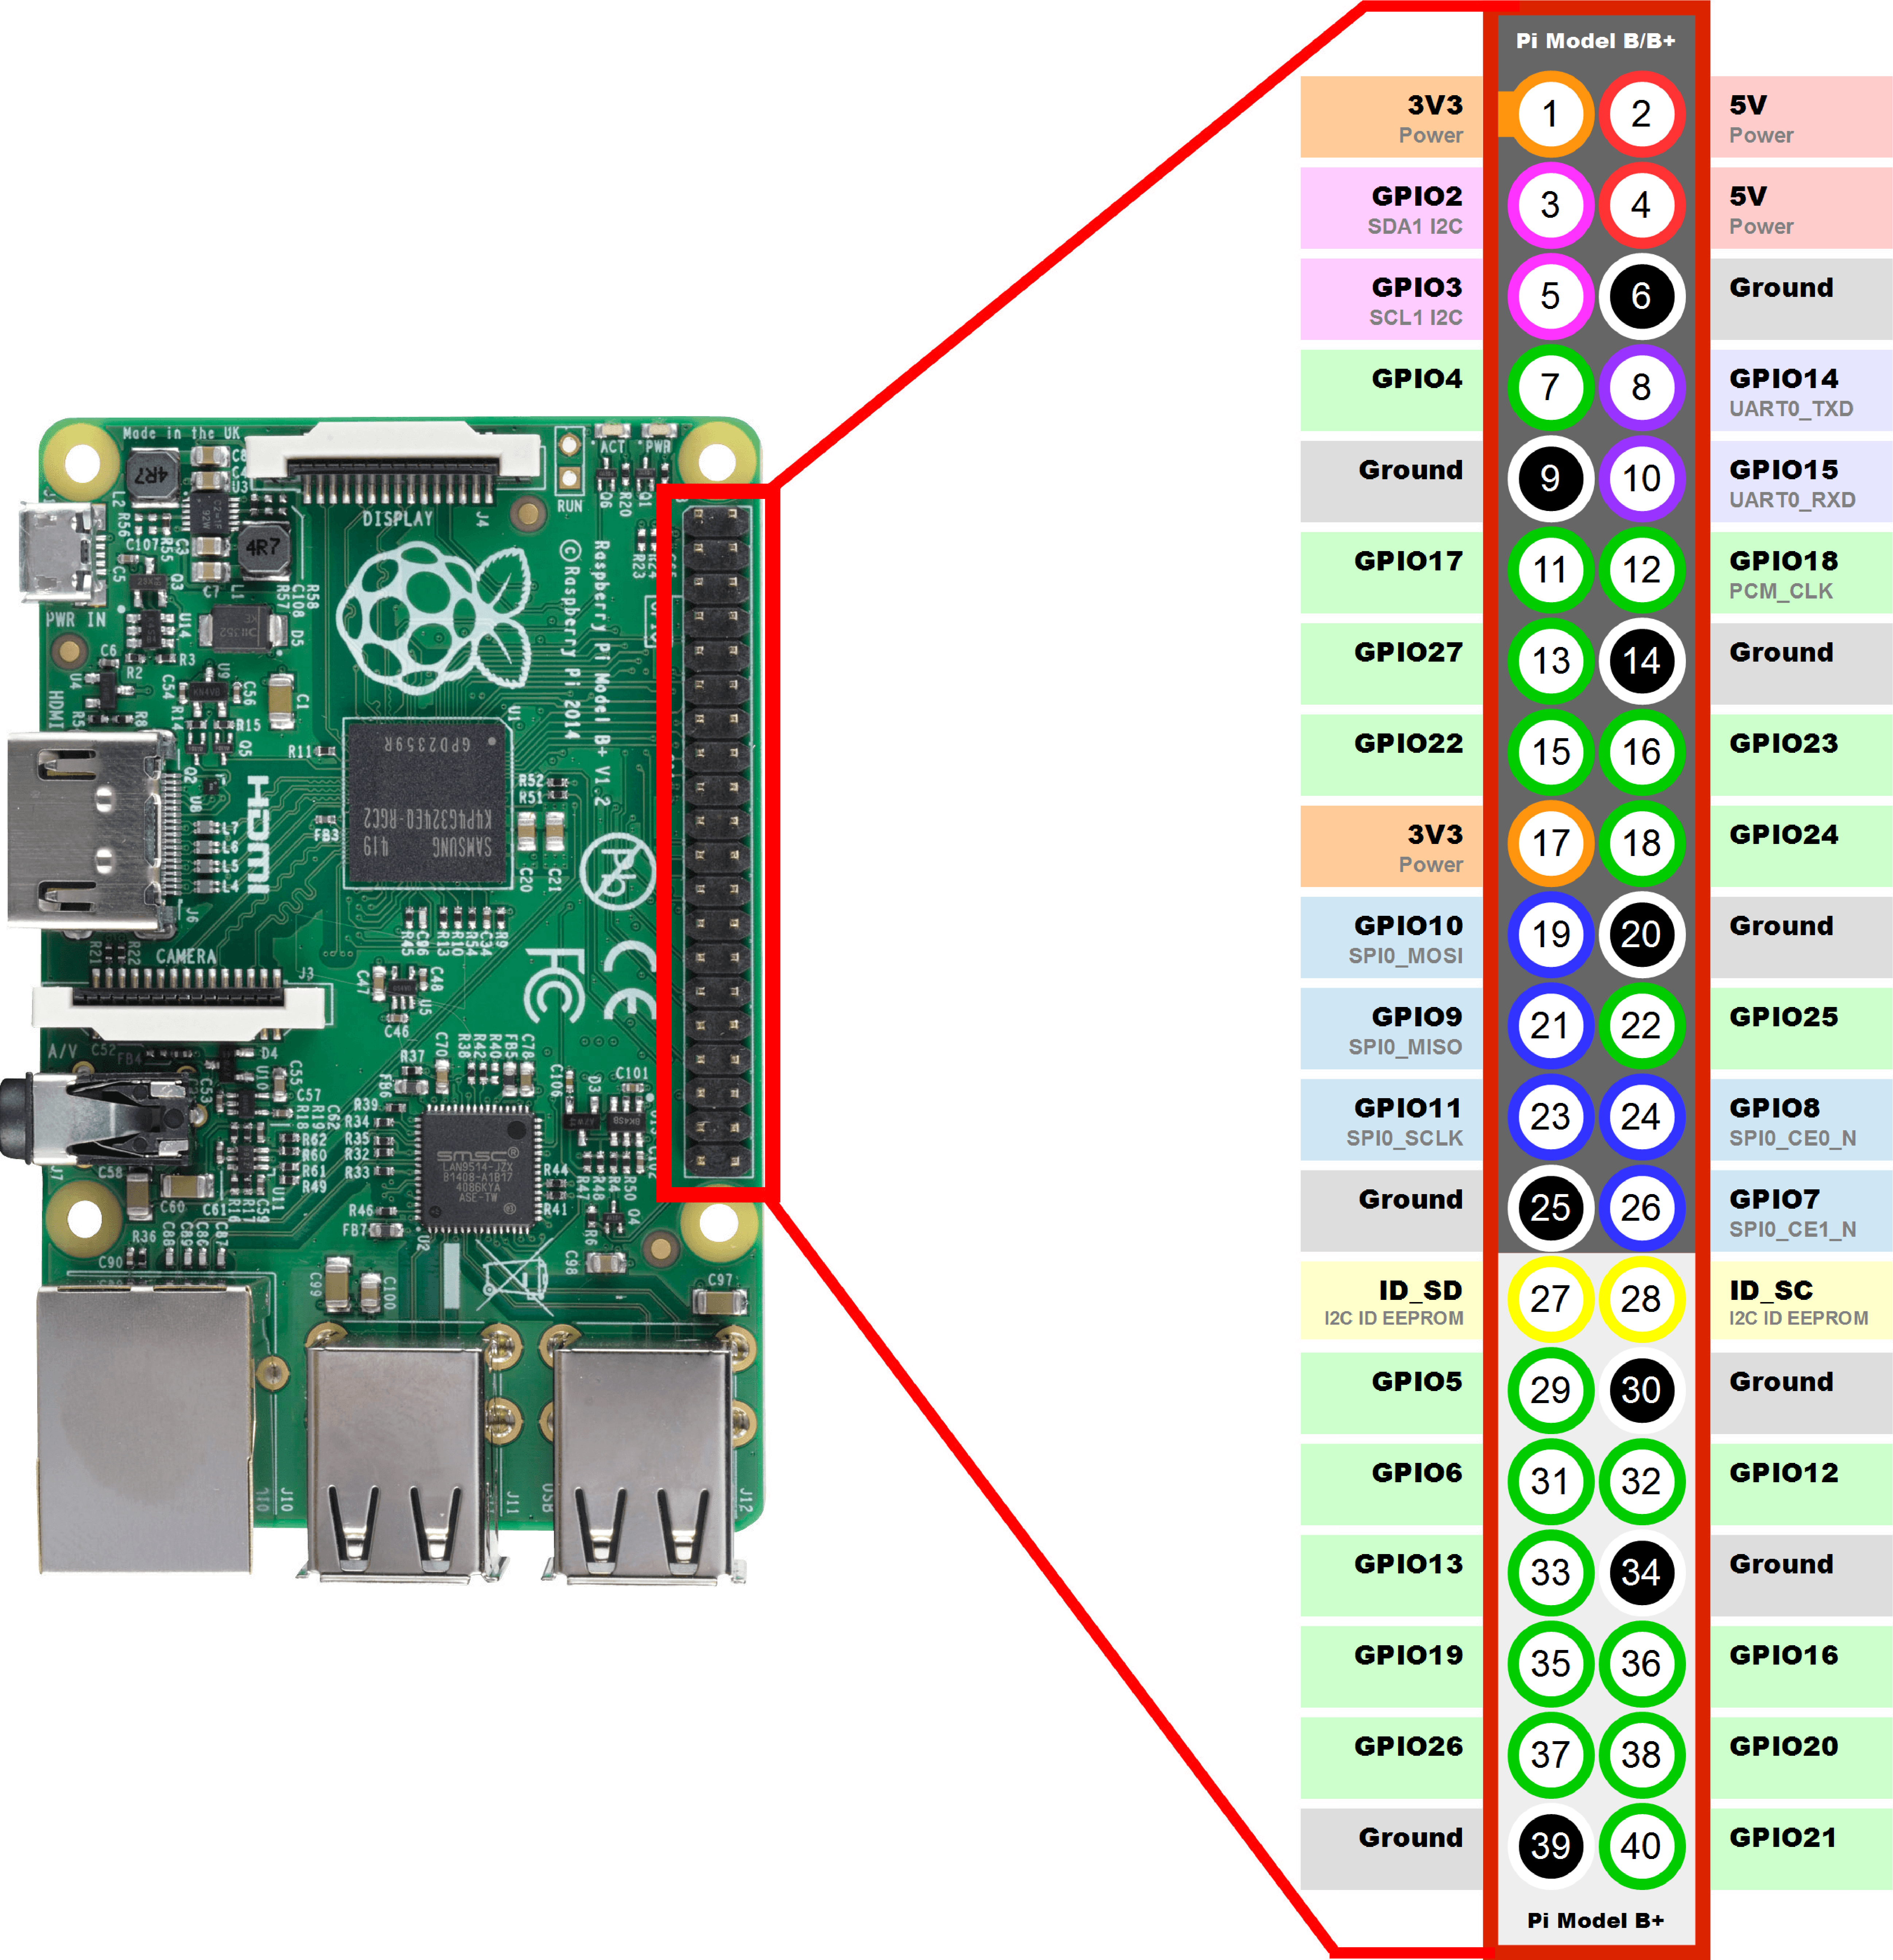
\includegraphics[scale=0.15, angle=0]{img/gpio.pdf}}
		\caption{Назначение пинов Raspberry Pi 2B}
		\label{pic:gpio}
	\end{center}
\end{figure}

Пин GPIO имеет два режима:
\begin{itemize}
	\item \textbf{Вход}. Напряжение подаётся внешним устройством. От +0.0В до +1.8В считается уровнем логического нуля, +1.8В-3.3В - логическая единица.
	\item \textbf{Выход}. Напряжение подаётся самим Raspberry Pi. Уровень логических 0 и 1 аналогичный.
\end{itemize}

По сути, передача и приём информации осуществляется только считыванием и установлением определённого напряжения. Выходы, отмеченные на схеме зелёным цветом имеют наиболее простой принцип действия: режим ввода/вывода в них устанавливается на всё время подключения устройства, а значение напряжения является относительно постоянным, так как по ним передаётся минимальное количество информации. 

В отличие от них, контакты имеющие подпись I2C, SPI или UART используются для последовательный синхронной передачи данных в режиме полного или полудуплекса. Это означает, что они используются для передачи уже более большого количества данных и могут переключать режим ввода/вывода по несколько тысяч раз за секунду. 

Целью данной работы является разработка базового взаимодействия с внешними устройствами, поэтому  ПО будет ориентировано на более простые интерфейсы GPIO.

\subsection{Анализ способа передачи информации}
Следующей задачей является определение способа и формата данных в передаче информации интерфейсу GPIO.

Для работы с пинами используется отображение в память (memory maping). Для чтения или изменения состояния устройства требуется взаимодействовать с определённым участком оперативной памяти, имеющей постоянный физический адрес. 

Рассмотрим устройство отображения GPIO в память для Raspberry Pi 2B. В листинге \ref{lst:mapping_const} приведены используемые константы\cite{subj:gpio_addr}.
\begin{lstlisting}[caption = {Адреса отображения в память}, label=lst:mapping_const]
	#define BCM2708_PERI_BASE	0x3F000000
	#define GPIO_BASE           (BCM2708_PERI_BASE + 0x200000) 	
	/* GPIO register offsets */
	#define GPFSEL0		0x0		/* Function Select */
	#define GPSET0		0x1c	/* Pin Output Set */
	#define GPCLR0		0x28	/* Pin Output Clear */
	#define GPLEV0		0x34	/* Pin Level */
	...
\end{lstlisting}

Адрес \textbf{BCM2708\_PERI\_BASE} определяет начало участка memory mapping для периферийных устройств, участок GPIO имеет смещение $0x200000$. Далее представленны смещения участков памяти относительно базового адреса \textbf{GPIO\_BASE}, каждое из которых отвечает соответственно за режим ввода/вывода, установку, сброс и чтение значения с пинов.


\subsection{Структура загружаемого модуля ядра}
Доступ к физической памяти возможно получить только режиме ядра. Поэтому, для выполнения постановленной задачи требуется написать загружаемый модуль ядра. После загрузки он становится частью ОС и получает доступ к ядрёным функциям и к памяти устройств ввода/вывода, что и требуется в этом случае. 

Для обеспечения доступа к устройствам принято решение использовать символьное устройство. Набор возможных действий с ним определяется структурой file\_operations, которая частично приведена в листинге \ref{lst:struct_op}.
\begin{lstlisting}[caption = {Структура file\_operations}, label=lst:struct_op]
struct file_operations {
	struct module *owner;
	...
	long (*unlocked_ioctl) (struct file *, unsigned int, unsigned long);
	...
	int (*open) (struct inode *, struct file *);
	int (*release) (struct inode *, struct file *);
	...
};
\end{lstlisting}

Взаимодействие с устройствами фактически производится через функцию unlocked\_ioctl. Для её вызова используется функция \textbf{ioctl}. В качестве аргументов передаётся структура открытого файла символьного устройства, номер команды и указатель на данные ввода или вывода. Для задания номеров команд используются макросы описанные в листинге \ref{lst:iowr}. Наличие R или W в названии указывают на то, что операция направленна на вывод или ввод соответственно. В качестве аргументов подаются тип и размер передаваемых данных, а также \"магическое число\" (уникальное число, позволяющее обнаружить ошибки некорректности команды с помощью макроса \textbf{\_IOC\_TYPE}).

\begin{lstlisting}[caption = {Макросы команд ioctl}, label=lst:iowr]
_IO(type,nr);
_IOR(type,nr,size);
_IOW(type,nr,size);
_IOWR(type,nr,size);
\end{lstlisting}

ПО должно предоставлять минимальные необходимые функции для управления контактами:
\begin{itemize}
	\item ввод / вывод значений;
	\item захват / возвращения управления пином;
	\item установление режима работы.
\end{itemize} 

Такие операции как захват и возврат управления нужны для того, чтобы обеспечить монопольный доступ на изменение для одного процесса. Таким образом, без управления пином возможно только чтение его значения.

\subsection{Получение памяти ввода/ввода}
Для того, чтобы память ввода/вывода стала доступной для использования модулем, требуется вызвать функции представленные в листинге \ref{lst:get_memory} \cite{subj:memory}.

\begin{lstlisting}[caption = {Получение доступа к памяти IO}, label=lst:get_memory]
	struct resource *request_mem_region(unsigned long start, unsigned long len, char *name);
	void *ioremap(unsigned long phys_addr, unsigned long size);
	u32 readl(const volatile void __iomem *addr);
	void writel(u32 b, volatile void __iomem *addr);
\end{lstlisting}

С помощью функции \textbf{request\_mem\_region} производится выделение участка физической памяти для использования модулем. Однако, данный участок памяти не будет доступен напрямую. Для его использования требуется вызвать функцию \textbf{ioremap}. Она возвращает виртуальный адрес, который используется для получения доступа к физическому. Чтение и запись из такого адреса производится через команды \textbf{readl}, \textbf{writel}.

\subsection*{Вывод}
\addcontentsline{toc}{subsection}{Вывод}
В этом разделе были сформулированы цель и задачи, выделены функции. Изученны особенности интерфейса GPIO. Было принято решение использовать символьное устройство для управления устройствами.
